\documentclass{article}

\usepackage[utf8]{inputenc}
\usepackage{setspace}
\usepackage[
	a4paper,
	total={17cm,25cm},
	top=3cm, left=2cm,
	includefoot
	]{geometry}
\usepackage[
	english,
	czech
	]{babel}
\usepackage[autostyle]{csquotes}
\usepackage{caption}
\usepackage{graphicx}
\graphicspath{{./assets/}}

\title{Návrh hry - Blokranč}
\author{Petr Maronek}
\date{5.11.2022}

% 	Vysvětlivky
%	\section* hvězdička znamená, že má LaTeX odebrat číslování

\begin{document}
	\begin{spacing}{1.15}
		\rmfamily
		\maketitle
		\begin{center}
			\textbf{Vysoká škola finanční a správní}\linebreak
			Fakulta právních a správních studií\linebreak
			Návrh počítačových her\linebreak
			Zimní semestr 2022\linebreak
			Vedoucí práce: \textbf{doc. Ing Stanislava Mildeová CSc.}
		\end{center}
		\pagebreak
			
		\section*{Abstrakt}
		Hra v prohlížeči na bázi těžby herních prostředků, která umožňuje hráči reálně zhodnocovat své majetky v herním prostředí. Pomocí herních tokenů může zdokonalovat své NFT nástroje, které těží více těchto tokenů. Tokeny a NFT se poté dají prodat na trhu za reálnou hodnotu.
				
		\section*{Klíčová slova}
		krypto, NFT, farma, playToEarn, prohlížeč
		\pagebreak
		    
		\section*{Úvod}
		Blorač je hra postavená na \textbf{blockchain} technologii. Bude splňovat takzvaný model "Play To Earn" což se dá volně přeložit jako "Vydělej si hraním". Do těchto typů her je nicméně nutná počáteční investice reálných peněz na nákup tokenů potřebných k nákupu či vyrobení si nezbytných nástrojů k hraní hry. 
		
		\section*{Myšlenková mapa}
		V této části práce se zaměřím na prvky hry, které budou hrát nejdůležitější roli. Níže zobrazuji tyto prvky formou myšlenkové mapy, kde značím stěžejní pilíře hry.
		
		\begin{center}
			\label{Myšlenková mapa}
			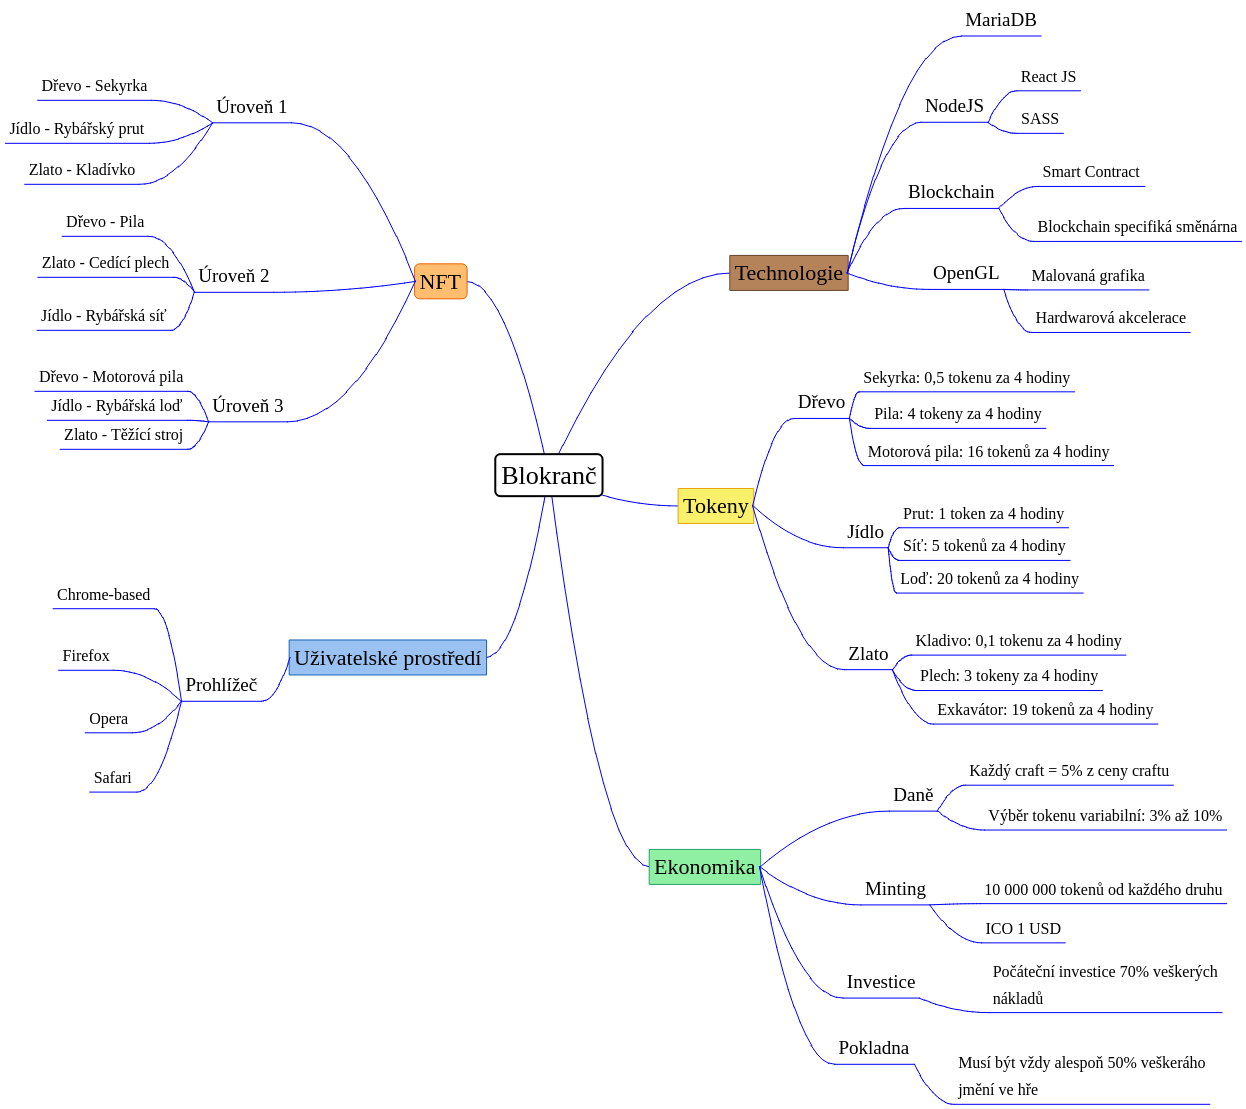
\includegraphics[scale=0.5]{221104-NPH-Blokranč.png}
			\captionof{figure}{Myšlenková mapa}
		\end{center}
		
		
		A pokračujeme v textu dál.
	
	\end{spacing}
\end{document}

